\section{You Only Look Once}

Il nome "You Only Look Once" deriva dalla filosfia di design che sta alla base del modello ideato da Joseph Redmon, Santosh Divvala, Ross Girshick e Ali Farhadi nel 2016\cite{14}: l'immagine deve essere elaborata una sola volta per effettuare sia la predizione delle bounding box che la classificazione degli oggetti. A differenza dei modelli two-stage, che richiedono un primo passaggio per generare le region proposals e un secondo passaggio per classificarle, YOLO effettua tutto in un unico passo. Questo approccio consente di ridurre drasticamente il tempo di elaborazione e semplifica l'architettura complessiva del modello.

Esistono quindi alcuni principi chiave che hanno influenzato il design e lo sviluppo del modello:
\begin{itemize}
  \item \textbf{Approccio Globale all'Immagine}: A differenza dei modelli precedenti che esaminano porzioni dell'immagine in sequenza, YOLO considera l'intera immagine in un singolo passaggio. Questo consente al modello di avere una visione globale del contesto, riducendo la probabilità di predizioni incoerenti tra le diverse regioni dell'immagine.
  \item \textbf{Efficienza Computazionale}: YOLO è progettato per essere estremamente veloce. L'approccio single-shot consente di ridurre drasticamente il tempo di elaborazione, rendendolo adatto per applicazioni in tempo reale come la videosorveglianza, la guida autonoma e altre situazioni dove la velocità è critica.
  \item \textbf{Semplicità e Generalizzazione}:  La semplicità dell'architettura di YOLO non solo facilita l'implementazione, ma migliora anche la capacità del modello di generalizzare su diverse tipologie di immagini e scenari. Utilizzando un'unica rete neurale convoluzionale per predire sia le bounding box che le probabilità di classe, YOLO riesce a mantenere un equilibrio tra complessità e prestazioni.
\end{itemize}

\begin{figure}[ht]
    \centering
    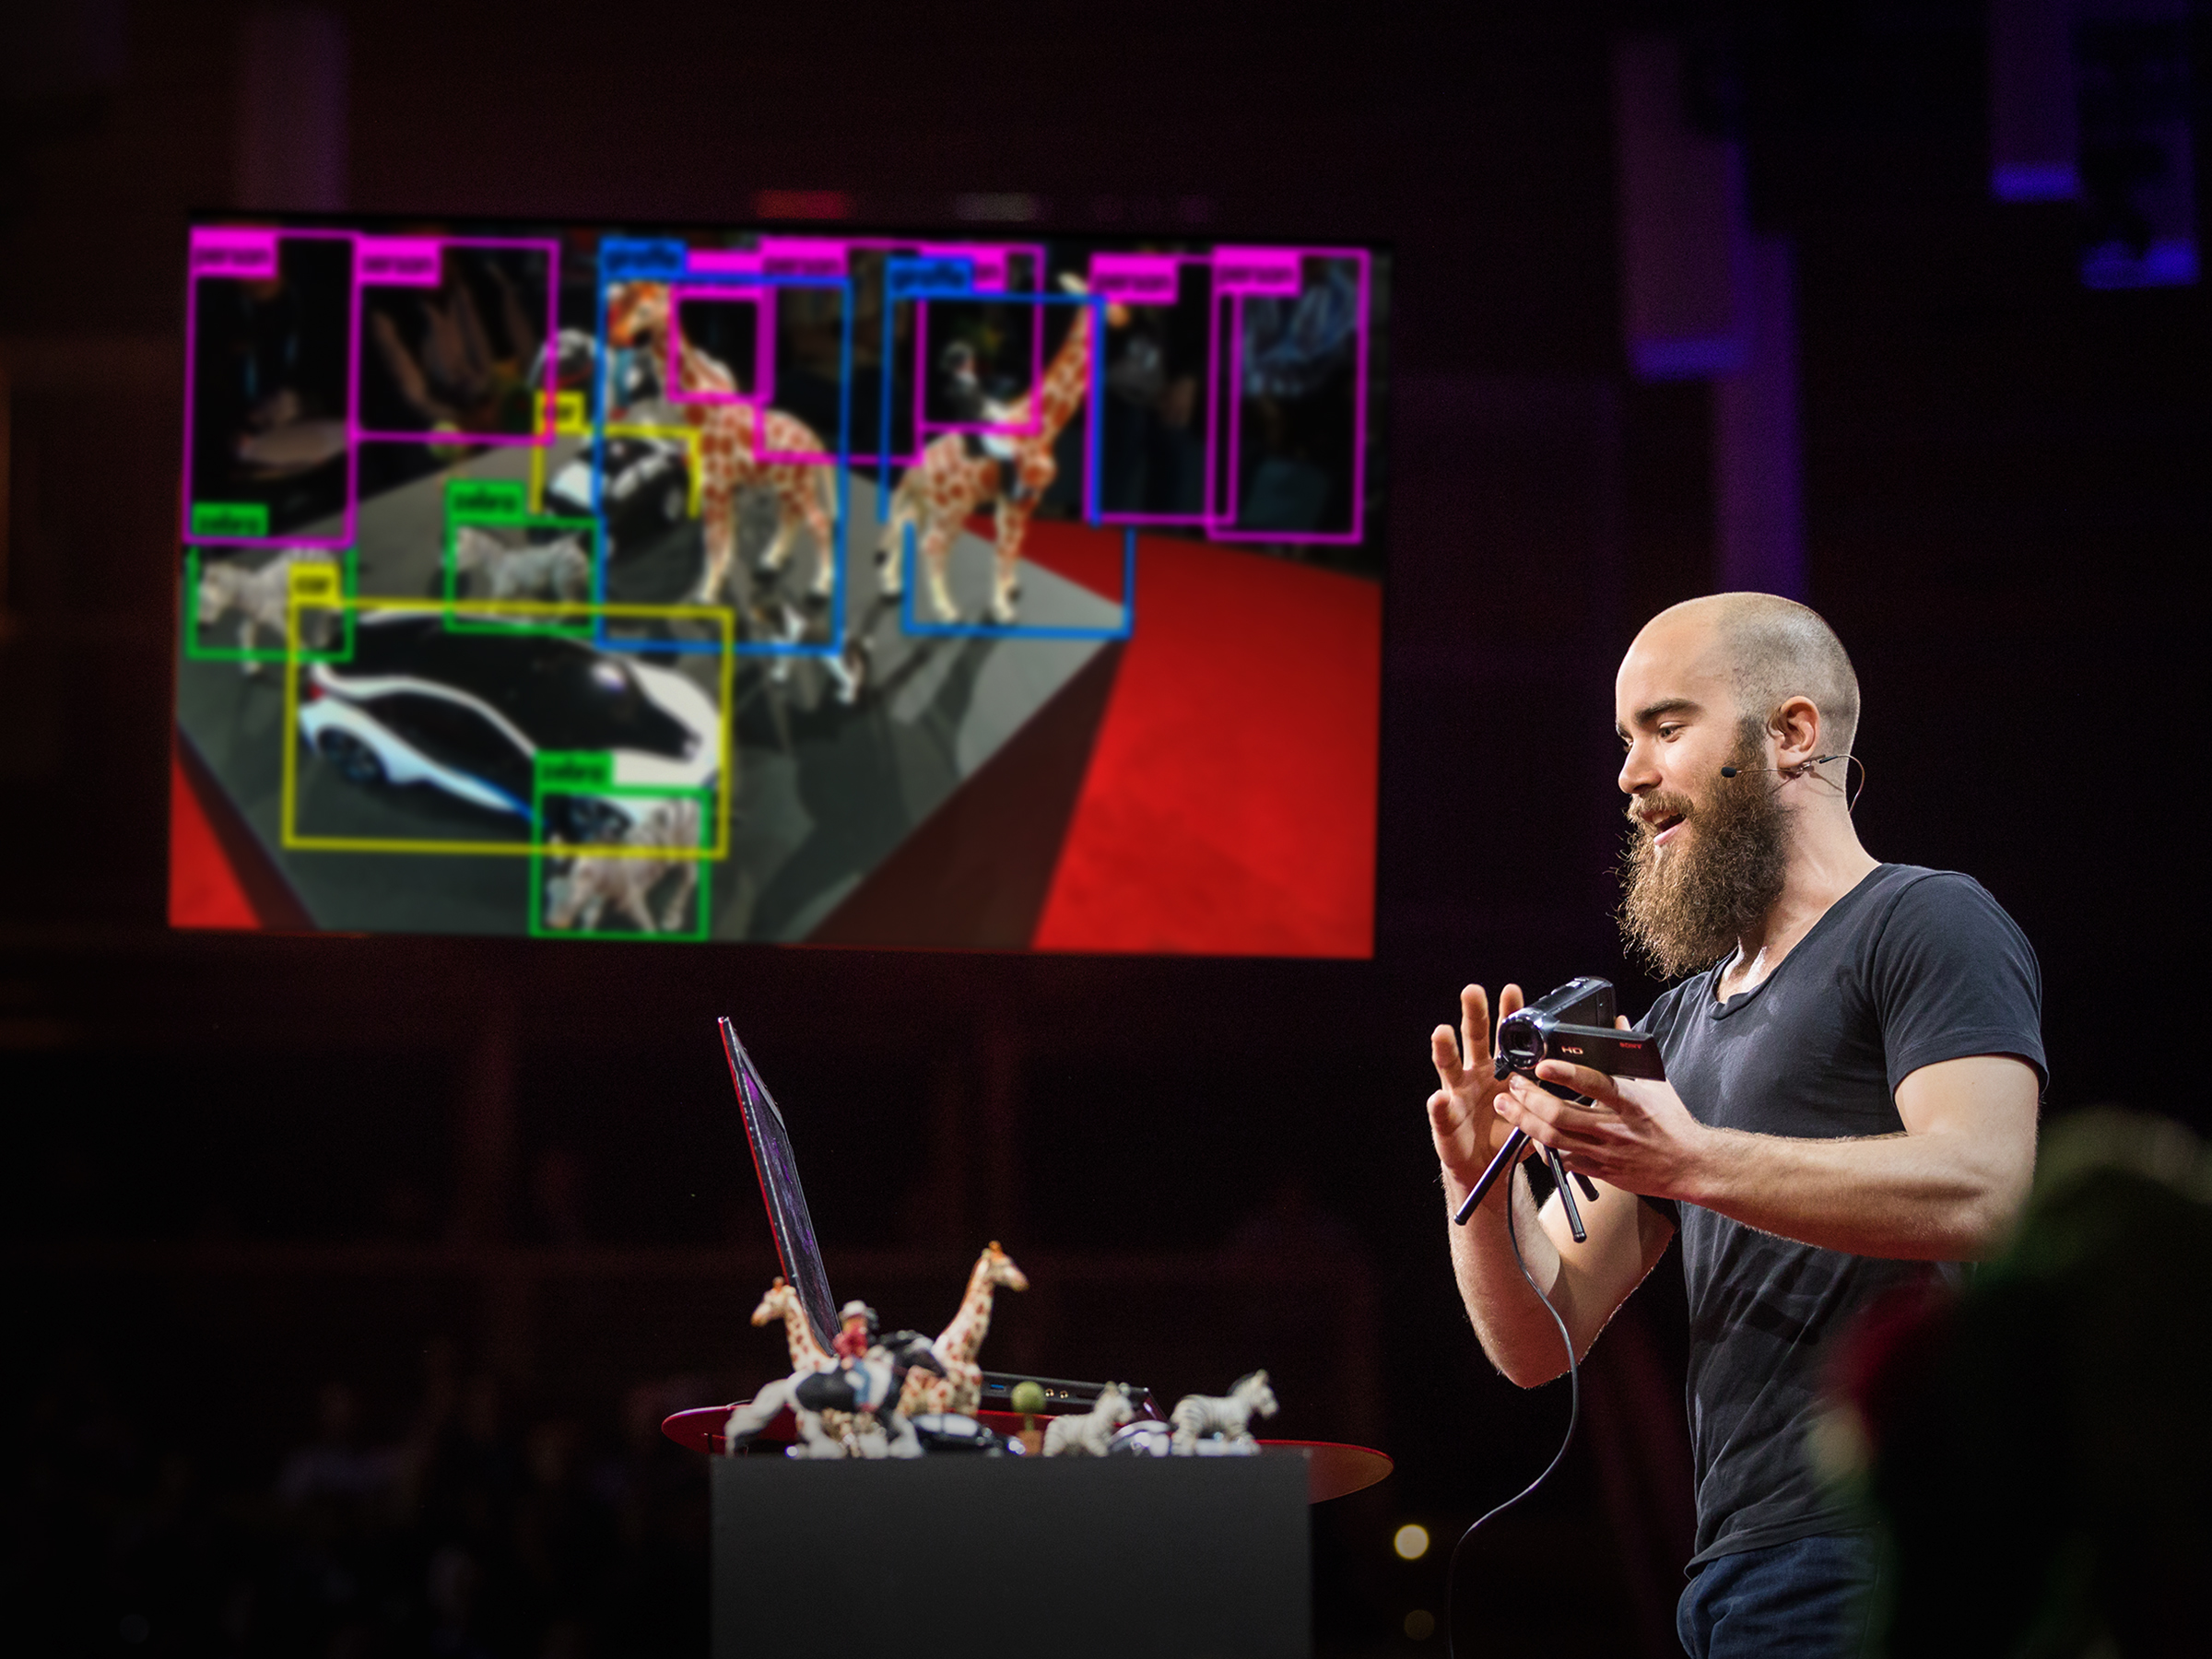
\includegraphics[width=0.8\textwidth]{files/capitoli/2-yolo/assets/joseph-redmon.jpeg}
    \caption{\label{fig:joseph-redmon}Joseph Redmon durante un TED Talk su YOLO nel 2017\cite{16}}
\end{figure}